\chapter{Lecture one: Introduction}

\section{Exam prerequisites and rules}

\begin{itemize}
    \item Written exam
    \item 4 hours duration
    \item Open book
    \item Computers are NOT permitted
    \item Internal censor
    \item Graded by the 7 point scale
\end{itemize}

\section{Workload}
\begin{itemize}
    \item Lectures - 24 hours
    \item Preparation - 48 hours
    \item Group exercises - 24 hours
    \item Submitted assignment - 21 hours
    \item Preparation for exam and trial exam - 33 hours
\end{itemize}

\section{System Development}
\begin{itemize}
    \item \textbf{Analysis:} Analysis and system requirements are analogous - the point is to find the unvarying requirements for a given system.
    \item \textbf{Design:} Work out a system design that has no major uncertainties.
    \item \textbf{Implementation:} Realise a specific design on a technical platform.
    \item \textbf{Method:} A guideline for working out system development activities, such as analysis, design, and implementation.
\end{itemize}

E.g. guidelines for work processes OOA\&D, and guidelines for documentation UML.

A method can be applied under different approaches, either the waterfall-method or the iterative-method. The writing of a book would be similar to the waterfall-method, as it's very hard not to write the given book sequentially.

\section{Object-Orientation}
An object is a single entity with an identity, a state, and some behaviour. An object belongs to a class.

A class is a description of a collection of objects sharing; structure, behavioural patterns, and attributes. Each class contains a set of objects - these are referred to to as objects of the class.

\subsection{Example with chair}
For a given dining-room chair some properties will relate to this object. The object will have an identity: myChair, a state: by dining table, not stuck, behaviour: bought, moved to, ... , sat down on, got up from, sold.

Seing a chair as a class, all chairs, as objects, will have some structure, namely an owner, attributes, positions, state (whether used or not). Behavioural pattern: \texttt{buy + \{move | sit down on + get up from\}* + sell}.

\subsection{Example with warehouse}
A warehouse is a large collection of articles stored in separate positions. Some way of defining positions of these articles is needed.

An article can be entered into, moved within, and removed from the warehouse. 

An article as an object, has an identity (barcode), state (placement in warehouse), behavioural properties (intake, moved around the warehouse, outtake).

Examples of classes in a warehouse could be:
\begin{itemize}
    \item Pallets
    \item Goods
    \item Boxes
    \item Employees
    \item Managers
\end{itemize}

\subsection{Example with gravel pit}
A class of materials has an identity (namely the type of material), state (current position, speed, wetness), behavioural patterns (dug up, moved to, moved from).

\begin{itemize}
    \item Tools
    \item Grading machines
    \item Pile
    \item Grain
    \item Material
    \item Rocks
\end{itemize}

You can discuss whether a box is a whole pallet or just a single box. 

If we had to model the gravel pit, we would have to decide on what kind of object we'd model the material as. As we're indifferent to the particular piece of grain, we're able to simplify the structure by granulating it into piles of a specific material. E.g. a pile of fine sand, a pile of clay, etc. These piles would then have an identifier as an identity, weight, and probably dimensions of the pile as state-information. Behavioural patterns would be piling material on, shovelling material out, etc.

\section{Objects in Analysis and Design}
\textbf{Analysis} concerns phenomena outside the computer system. Identity in this sense identifies a specific object. Behaviour are the events an object has performed or been subjected to. 

\textbf{Design} (and implementation) concerns phenomena inside the computer system. Identity is the description of how to get access to an object.
Behaviour is the operations an object can perform on request and offer to other objects.

\section{Model the Context}
Focus on an IT system and its context. The \textbf{problem domain} is then the part of a context that is administrated, monitored, or controlled by a system. The \textbf{application domain} is the organisation that administrates, monitors, or controls a problem domain. The system is contained within this application domain.

\section{Model of a problem domain}
\begin{figure}
    \centering
    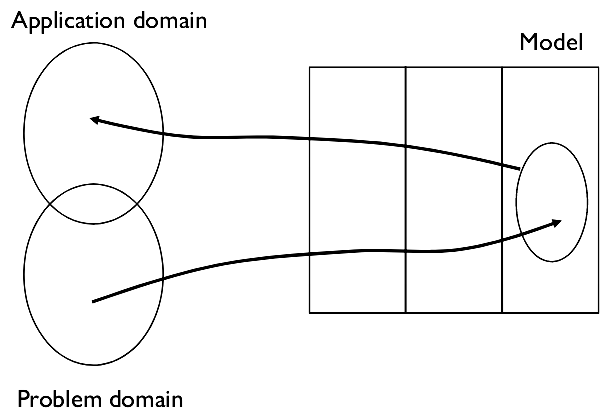
\includegraphics[width=0.6\textwidth]{figures/problemdomain.png}
    \caption{Problem domain model}
    \label{fig:problemdomainmodel}
\end{figure}

The \textbf{model}, figure \ref{fig:problemdomainmodel}, is an updated representation of the state in the problem domain. When something happens in the problem domain, e.g. a new chair is taken into a warehouse, we then register that in our model, so that it is known that we've got an extra chair. A \textbf{user} is in the application domain and gets information about the problem domain mediated through the model. 

\subsection{Example of a AAB-problem domain model}
In the application domain we've got the users that utilise the system, which presents and stores information about the team, players, and related information. The problem domain is all relevant information and actions, injuries, red/yellow cards and the like. Whenever this information changes, then a change in the model is required. Sometimes this is automated, sometimes is a manual action.

The system is then composed of a UI, which is the only thing that users see, an assorted collection of functions that transforms this data, and finally the model of the given problem domain.

\begin{figure}[h]
    \centering
    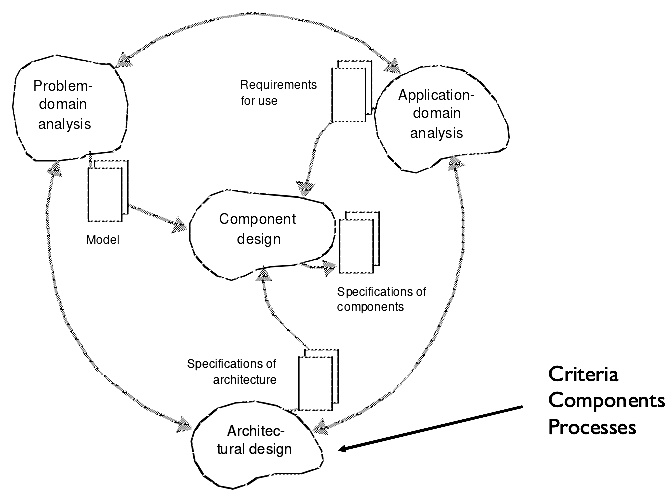
\includegraphics[scale=1.5]{figures/methodcircular.png}
    \caption{The method}
    \label{fig:methodcircular}
\end{figure}

\section{The \ad-method}
Class, structure, and behaviour relates to the problem-domain analysis. Usage, functions, and interfaces relates to the application-domain analysis. Criteria, components, and processes relates to architectural design. Lastly model component, function component, and connecting components relate component design. This is shown in figure \ref{fig:methodcircular}.

\begin{figure}[h]
    \centering
    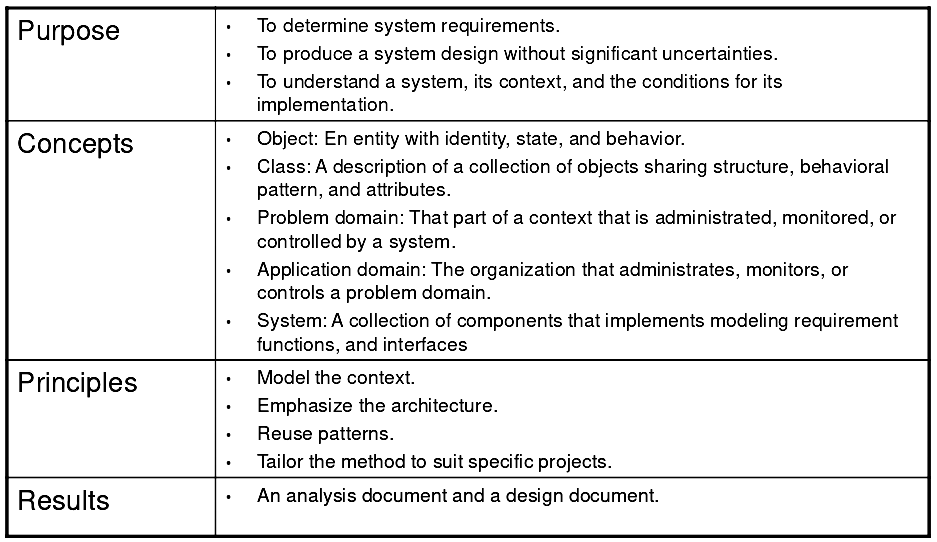
\includegraphics[width=0.75\textwidth]{figures/ooadmedthodsummary.png}
    \caption{The \ad method}
    \label{fig:methodcircular}
\end{figure}

\section{System choice}
A system definition explains all relevant areas of a given systems function and is meant to agree on the overall system characteristics. This results in a system definition that fulfils the FACTOR criterion.
The question of this activity is; \textit{should this class be included or not?}

\subsection{Situation}
Our understanding of the users' situation much be rich and abundant. In achieving this, it's important to be open and disposed toward discussion. Therefore; \textit{appreciate the situation.}

\subsection{Rich pictures}
A rich picture is an informal drawing that presents the illustrator's understanding of the situation. A rich picture focuses on the important aspects of the situation but should give a broad description of the situation that enables several alternative interpretations.

\subsection{Ideas}
Having a solid understanding of the existing situation is a good starting point for a development project. It's just as important to bring forth new ideas and ways of thinking, though.

\subsection{Create ideas}
Creating ideas can be helped with the following methods.

\subsection{Metaphors}
Imagine the user organisation or computer-system through a new lens. This helps transfer ideas and experience from other areas to the development. 

A library could be interpreted as warehouse, a supermarket, or a school through metaphors. Meaning that looking up a position, taking stock, and getting directions are similar between libraries and warehouses.

Both looking at similar and dissimilar instances of metaphors is advantageous.

\subsection{Experiments}
An experiment is a planned examination of the target solution's properties. The experience should, more or less, resemble the users' daily work.

These experiments follow the systematic approach:

\begin{enumerate}
    \item Planning
    \item Development
    \item Preparation
    \item Test
    \item Summarising
\end{enumerate}

\section{Systems}
The purpose of the third and final subactivity is to choose the actual system to develop. This is done by systematically clarifying interpretations, possibilities, and consequences of several alternative solutions. Hence, the following principle; \textit{define alternative systems.}

\section{System definition (FACTOR)}
The FACTOR criterion can be used in two ways; to either support system-definition development or describing the system and then use the criteria to see how the system definition satisfies each of the six factors. Both are equally viable.

\begin{itemize}
    \item[] \textit{Functionality:} The system functions that support the application-domain tasks
    \item[] \textit{Application domain:} Those parts of an organisation that administrate, monitor, or control a problem domain.
    \item[] \textit{Conditions:} The conditions under which the system will be developed and used.
    \item[] \textit{Technology:} Both the technology used to develop the system and the technology on which the system will run.
    \item[] \textit{Objects:} The main objects in the problem domain.
    \item[] \textit{Responsibility:} The system's overall responsibility in relation to its context.
\end{itemize}

Getting the system definition right and quick is important for all further activities. Often the system definition will iteratively be revised during \ad.

\subsection{Difficulties with system definition elements}
\textbf{Functionality and responsibility} is quite similar, however, functionality are the means to achieve the responsibility of a given system. In the greenhouse-example, updating and recording temperature versus display or control.
\textbf{Technology and conditions.} Technology is the actual tech used to develop the system and the hardware that the system will run on. Conditions are quite simply under which restraints, and conditions are this development made, e.g. in collaboration with professional or with cheapest possible hardware.

\subsection{Understanding responsibilities}
The system is responsible for certain things, which the user is not - and vice versa. Although, some of these tasks can be moved between the system and user, e.g. an autopilot on a plane.

\subsection{Evaluation and choice}
It is not the system developers' job to choose a system; your job is to facilitate choice. Active negotiation between involved parties is essential, if the system is to persevere. The choice of system should be made at an early stage, which has several implications. First, later insight may lead to changes. It's important to iterate during system choice, since describing the situation and generating ideas are so tightly tied to formulating and choosing the system definition, these subactivities cannot be completed until the final choice is made. Lastly, ensure that all parties understand the implications of what they choose at this early stage.

During this process, it's important to question arguments. Always try to base arguments on documented facts, such as \textbf{rich pictures} or \textbf{prototype evaluations}. Fundamental conflicts may also exist, and they do not disappear just because we try to avoid them. Therefore; 
\begin{center}
    \textit{we must resolve conflicts or suffer the consequences}
\end{center}

\subsection{Summary}
\begin{figure}[H]
    \centering
    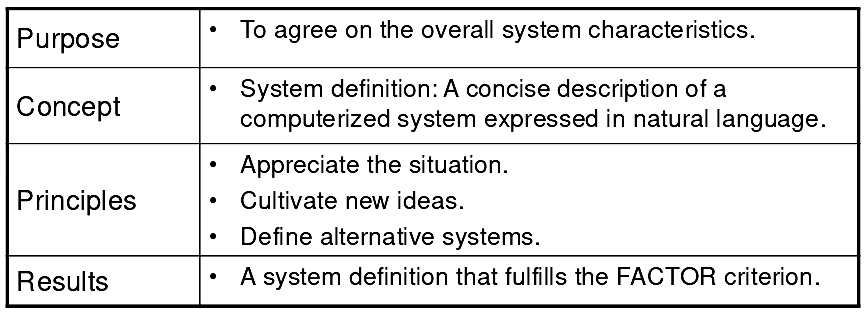
\includegraphics[width=0.75\textwidth]{figures/systemchoicesummary.png}
\end{figure}

\section{Exploring alternative system definitions}
System developers explore different alternative systems by changing elements of the system definition. E.g. with a bank, old-school banking versus modern, networked banking. Evaluate which and why the user might want either version.

\subsection{Conference administration}
Func = \textit{functionality}. Resp = \textit{responsibility}.
\begin{itemize}
    \item[Func 1] Register information about participants and produce a complete participant list
    \item[Func 2] Register general participants as well as those with an active role such as author, speaker, or reviewer. Support the administration of finances and invitations. Support development of conference programs, including registration, paper acceptance, and sessions division.
    \item[Resp 1] Support program design by producing overviews and allowing users to add components and save difference versions. Support conference operations by emphasising potential problems at regular intervals.
    \item[Resp 2] Automatic conference-planning program. Generate program from suggested sessions and incoming paper reviews.
\end{itemize}

\subsection{Principles}
\subsubsection{Appreciate the situation}
The customer's or users' understanding of the task is an important starting point. But you should also look behind their formulations and understand the situation in which the new system will be used. Rich pictures provide a quick overview of complex and ambiguous situations. They are a good basis for discussion and give us a way to express different interpretations of the same situation. 

\subsubsection{Cultivate new ideas}
Every development project is an opportunity to take a critical look at established traditions and think in new and different ways. Exemplars, metaphors, and exploratory experiments are cheap and effective techniques to bring new ideas into play.

\subsubsection{Define alternative systems}
The customer and users are responsible for choosing the solution. System definitions are brief and concise descriptions of possible alternatives that can serve as a basis for their evaluation of possibilities and their choice of a satisfactory solution.

\section{Exercises}
\begin{itemize}
    \item Write text for each element of the FACTOR criterion
    \item Introduce variations on selected elements
    \item If relevant, write the FACTOR criterion as a coherent piece of text
\end{itemize}
\subsection{Quiz}
22 minutes duration, 87\% correct answers.